\begin{figure}[p]\centering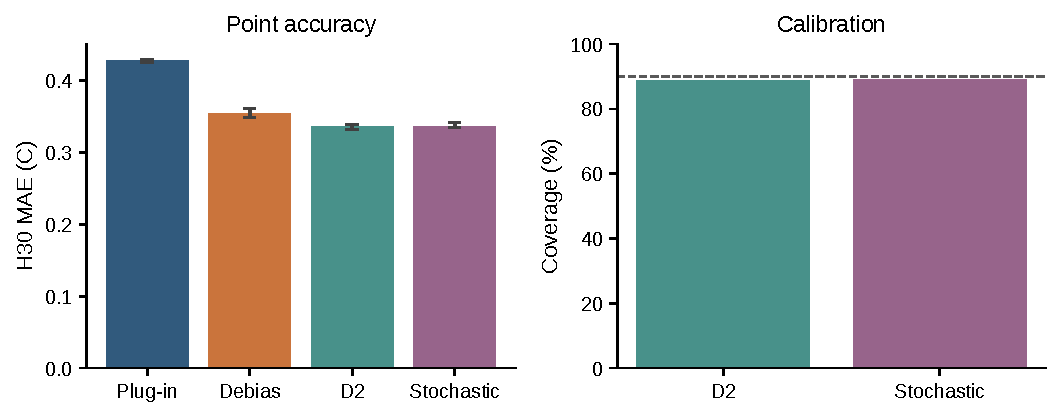
\includegraphics[width=\textwidth]{figures/simple_research/02_annual_comparators.pdf}\caption{Annual estimation under difficult controlled gaps. Both historical source-calibrated methods receive the same observed-bound projection and normal-spacing tail model. Bars show empirical repetition ranges within the same archive; these are not independent climates.}\label{fig:estimators}\end{figure}
\begin{figure}[p]\centering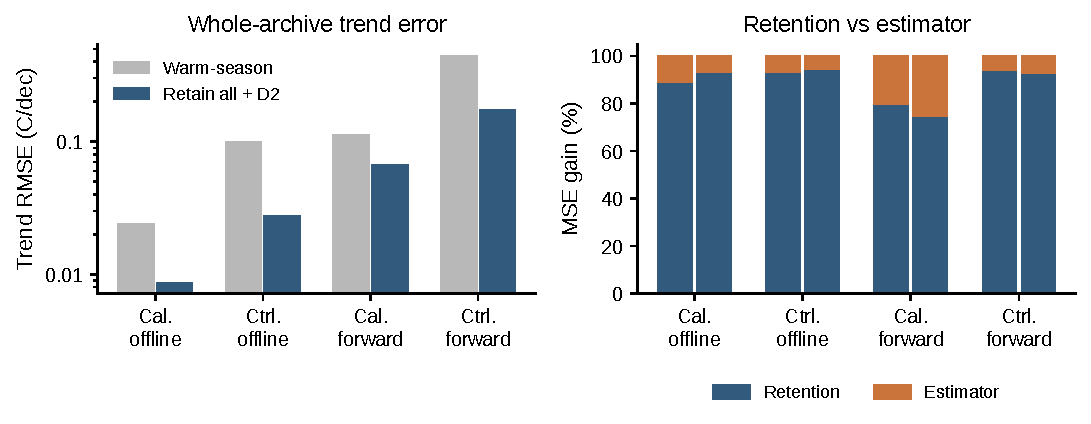
\includegraphics[width=\textwidth]{figures/simple_research/03_archive_factorial.pdf}\caption{Whole-archive trend errors and the symmetric retention/estimator decomposition. Left: D2 on common station-repetition rows where both retention sets are available; annotations give n and station/group counts. The forward controlled-gap contrast uses 807 of 820 settings. Right: the left bar of each pair is D2 and the right bar is the calibrated classical method. Each bar uses that method's own complete four-cell count, printed under the setting; the two counts are not one shared denominator.}\label{fig:whole-archive}\end{figure}
\begin{figure}[p]\centering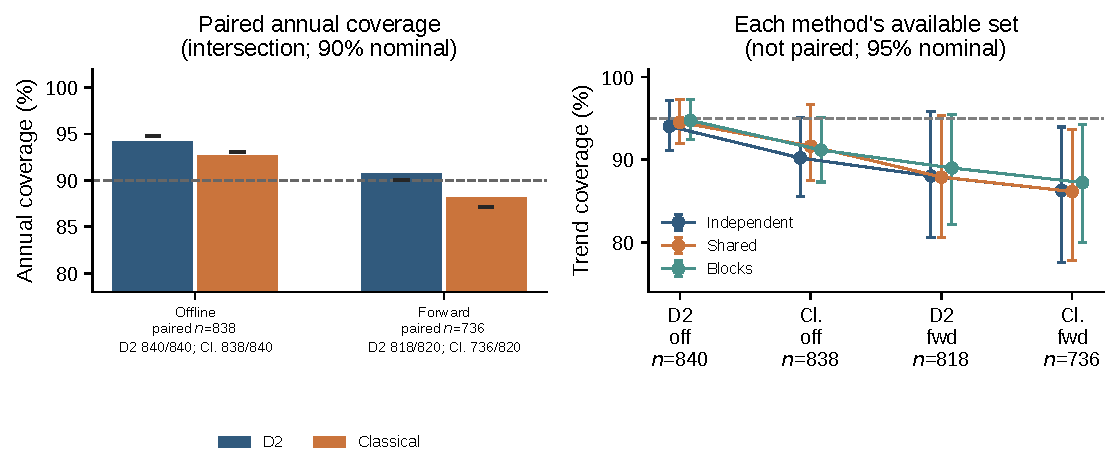
\includegraphics[width=\textwidth]{figures/simple_research/04_joint_uncertainty.pdf}\caption{Left: paired annual coverage on the two-method intersection, weighted by incomplete years. Ticks are station-repetition means on the same intersection. The tick labels give the paired archive count and each method's availability out of all archives. The dashed line is the nominal 90 percent annual target. Right: nominal 95 percent trend coverage on each method's own available archives, with that archive count. The right panel is not a paired method comparison. Group-bootstrap intervals use connected groups. No gray band is shown.}\label{fig:joint-uncertainty}\end{figure}
\begin{figure}[p]\centering
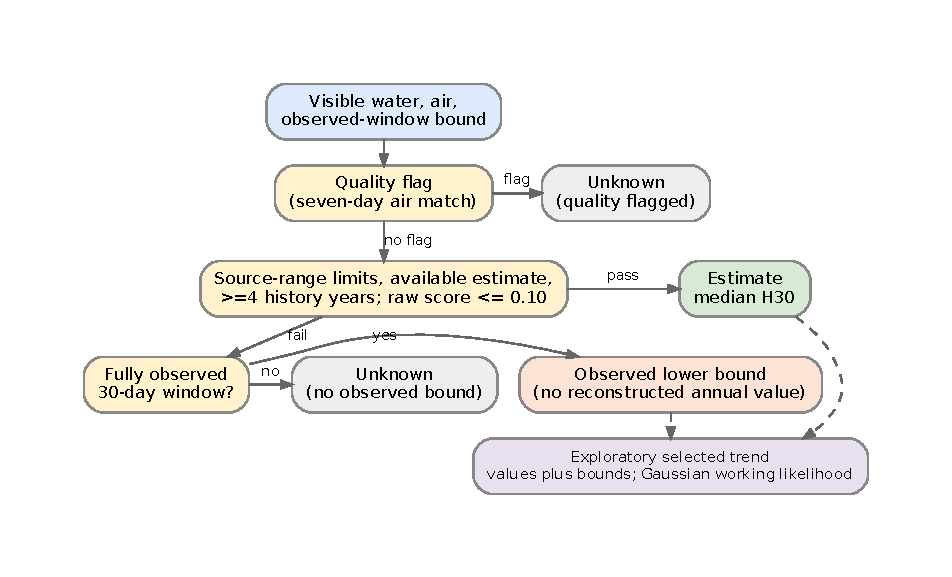
\includegraphics[width=\textwidth]{figures/architecture/fig2_release_actual.pdf}
\caption{The evaluated three-output decision and exploratory trend analysis. The cap applies to an individual raw classifier score, not a certified group risk. The seven-day water--air check was assessed only for the clean and imposed exact-air-substitution cases. The selected-trend working likelihood treats released values as exact and observed bounds as censored.}\label{fig:release-system}
\end{figure}
\begin{figure}[p]\centering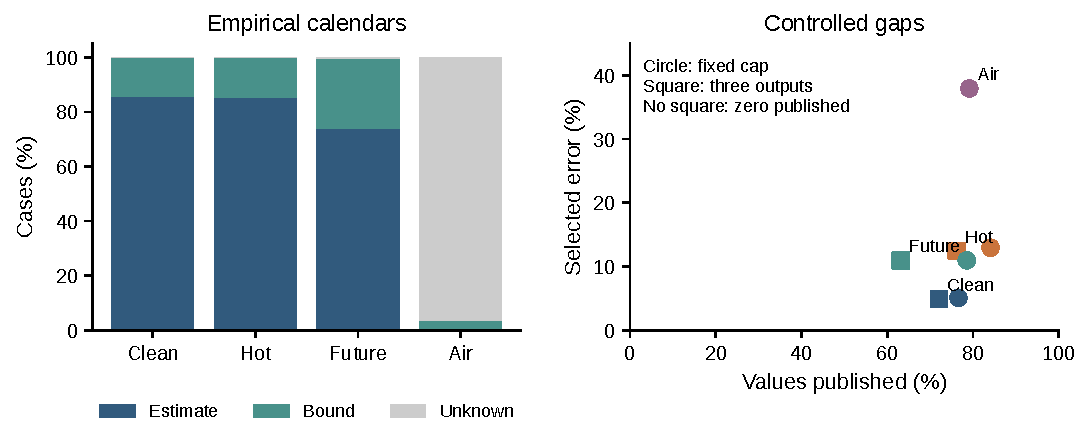
\includegraphics[width=\textwidth]{figures/simple_research/05_output_boundaries.pdf}\caption{Left: three outputs for empirical-calendar masks. Right: numerical-publication rates and selected errors for controlled gaps. Source diagnostics do not remove extrapolation failures. The air-agreement flag addresses the specified exact-substitution stress only; zero publication is shown as unknown rather than zero-risk success.}\label{fig:output-boundaries}\end{figure}
